% Options for packages loaded elsewhere
\PassOptionsToPackage{unicode}{hyperref}
\PassOptionsToPackage{hyphens}{url}
\documentclass[
]{article}
\usepackage{xcolor}
\usepackage[margin=1in]{geometry}
\usepackage{amsmath,amssymb}
\setcounter{secnumdepth}{-\maxdimen} % remove section numbering
\usepackage{iftex}
\ifPDFTeX
  \usepackage[T1]{fontenc}
  \usepackage[utf8]{inputenc}
  \usepackage{textcomp} % provide euro and other symbols
\else % if luatex or xetex
  \usepackage{unicode-math} % this also loads fontspec
  \defaultfontfeatures{Scale=MatchLowercase}
  \defaultfontfeatures[\rmfamily]{Ligatures=TeX,Scale=1}
\fi
\usepackage{lmodern}
\ifPDFTeX\else
  % xetex/luatex font selection
\fi
% Use upquote if available, for straight quotes in verbatim environments
\IfFileExists{upquote.sty}{\usepackage{upquote}}{}
\IfFileExists{microtype.sty}{% use microtype if available
  \usepackage[]{microtype}
  \UseMicrotypeSet[protrusion]{basicmath} % disable protrusion for tt fonts
}{}
\makeatletter
\@ifundefined{KOMAClassName}{% if non-KOMA class
  \IfFileExists{parskip.sty}{%
    \usepackage{parskip}
  }{% else
    \setlength{\parindent}{0pt}
    \setlength{\parskip}{6pt plus 2pt minus 1pt}}
}{% if KOMA class
  \KOMAoptions{parskip=half}}
\makeatother
\usepackage{color}
\usepackage{fancyvrb}
\newcommand{\VerbBar}{|}
\newcommand{\VERB}{\Verb[commandchars=\\\{\}]}
\DefineVerbatimEnvironment{Highlighting}{Verbatim}{commandchars=\\\{\}}
% Add ',fontsize=\small' for more characters per line
\usepackage{framed}
\definecolor{shadecolor}{RGB}{248,248,248}
\newenvironment{Shaded}{\begin{snugshade}}{\end{snugshade}}
\newcommand{\AlertTok}[1]{\textcolor[rgb]{0.94,0.16,0.16}{#1}}
\newcommand{\AnnotationTok}[1]{\textcolor[rgb]{0.56,0.35,0.01}{\textbf{\textit{#1}}}}
\newcommand{\AttributeTok}[1]{\textcolor[rgb]{0.13,0.29,0.53}{#1}}
\newcommand{\BaseNTok}[1]{\textcolor[rgb]{0.00,0.00,0.81}{#1}}
\newcommand{\BuiltInTok}[1]{#1}
\newcommand{\CharTok}[1]{\textcolor[rgb]{0.31,0.60,0.02}{#1}}
\newcommand{\CommentTok}[1]{\textcolor[rgb]{0.56,0.35,0.01}{\textit{#1}}}
\newcommand{\CommentVarTok}[1]{\textcolor[rgb]{0.56,0.35,0.01}{\textbf{\textit{#1}}}}
\newcommand{\ConstantTok}[1]{\textcolor[rgb]{0.56,0.35,0.01}{#1}}
\newcommand{\ControlFlowTok}[1]{\textcolor[rgb]{0.13,0.29,0.53}{\textbf{#1}}}
\newcommand{\DataTypeTok}[1]{\textcolor[rgb]{0.13,0.29,0.53}{#1}}
\newcommand{\DecValTok}[1]{\textcolor[rgb]{0.00,0.00,0.81}{#1}}
\newcommand{\DocumentationTok}[1]{\textcolor[rgb]{0.56,0.35,0.01}{\textbf{\textit{#1}}}}
\newcommand{\ErrorTok}[1]{\textcolor[rgb]{0.64,0.00,0.00}{\textbf{#1}}}
\newcommand{\ExtensionTok}[1]{#1}
\newcommand{\FloatTok}[1]{\textcolor[rgb]{0.00,0.00,0.81}{#1}}
\newcommand{\FunctionTok}[1]{\textcolor[rgb]{0.13,0.29,0.53}{\textbf{#1}}}
\newcommand{\ImportTok}[1]{#1}
\newcommand{\InformationTok}[1]{\textcolor[rgb]{0.56,0.35,0.01}{\textbf{\textit{#1}}}}
\newcommand{\KeywordTok}[1]{\textcolor[rgb]{0.13,0.29,0.53}{\textbf{#1}}}
\newcommand{\NormalTok}[1]{#1}
\newcommand{\OperatorTok}[1]{\textcolor[rgb]{0.81,0.36,0.00}{\textbf{#1}}}
\newcommand{\OtherTok}[1]{\textcolor[rgb]{0.56,0.35,0.01}{#1}}
\newcommand{\PreprocessorTok}[1]{\textcolor[rgb]{0.56,0.35,0.01}{\textit{#1}}}
\newcommand{\RegionMarkerTok}[1]{#1}
\newcommand{\SpecialCharTok}[1]{\textcolor[rgb]{0.81,0.36,0.00}{\textbf{#1}}}
\newcommand{\SpecialStringTok}[1]{\textcolor[rgb]{0.31,0.60,0.02}{#1}}
\newcommand{\StringTok}[1]{\textcolor[rgb]{0.31,0.60,0.02}{#1}}
\newcommand{\VariableTok}[1]{\textcolor[rgb]{0.00,0.00,0.00}{#1}}
\newcommand{\VerbatimStringTok}[1]{\textcolor[rgb]{0.31,0.60,0.02}{#1}}
\newcommand{\WarningTok}[1]{\textcolor[rgb]{0.56,0.35,0.01}{\textbf{\textit{#1}}}}
\usepackage{graphicx}
\makeatletter
\newsavebox\pandoc@box
\newcommand*\pandocbounded[1]{% scales image to fit in text height/width
  \sbox\pandoc@box{#1}%
  \Gscale@div\@tempa{\textheight}{\dimexpr\ht\pandoc@box+\dp\pandoc@box\relax}%
  \Gscale@div\@tempb{\linewidth}{\wd\pandoc@box}%
  \ifdim\@tempb\p@<\@tempa\p@\let\@tempa\@tempb\fi% select the smaller of both
  \ifdim\@tempa\p@<\p@\scalebox{\@tempa}{\usebox\pandoc@box}%
  \else\usebox{\pandoc@box}%
  \fi%
}
% Set default figure placement to htbp
\def\fps@figure{htbp}
\makeatother
\setlength{\emergencystretch}{3em} % prevent overfull lines
\providecommand{\tightlist}{%
  \setlength{\itemsep}{0pt}\setlength{\parskip}{0pt}}
\usepackage{bookmark}
\IfFileExists{xurl.sty}{\usepackage{xurl}}{} % add URL line breaks if available
\urlstyle{same}
% fallback for those not using the hyperref driver hyperxmp:
\makeatletter
\@ifundefined{xmpquote}{\newcommand{\xmpquote}[1]{#1}}{}
\makeatother
\hypersetup{
  pdftitle={Effect of Experimental Warming on Soil Bacterial Communities (soilrep dataset)},
  pdfauthor={2021/ASP/32},
  hidelinks,
  pdfcreator={LaTeX via pandoc}}

\title{Effect of Experimental Warming on Soil Bacterial Communities
(soilrep dataset)}
\author{2021/ASP/32}
\date{2026-11-12}

\begin{document}
\maketitle

{
\setcounter{tocdepth}{2}
\tableofcontents
}
\section{0. Packages}\label{packages}

\begin{Shaded}
\begin{Highlighting}[]
\CommentTok{\# Install once (uncomment if needed):}
\CommentTok{\# if (!require("BiocManager")) install.packages("BiocManager")}
\CommentTok{\# BiocManager::install(c("phyloseq", "DESeq2"))}
\CommentTok{\# install.packages(c("tidyverse", "vegan", "pheatmap"))}

\FunctionTok{library}\NormalTok{(phyloseq)}
\FunctionTok{library}\NormalTok{(DESeq2)}
\FunctionTok{library}\NormalTok{(vegan)}
\FunctionTok{library}\NormalTok{(tidyverse)}
\FunctionTok{library}\NormalTok{(pheatmap)}
\end{Highlighting}
\end{Shaded}

\section{1. Data import}\label{data-import}

\begin{Shaded}
\begin{Highlighting}[]
\CommentTok{\# Read the two CSV files stored in the repository\textquotesingle{}s data/ folder}
\NormalTok{otu  }\OtherTok{\textless{}{-}} \FunctionTok{read.csv}\NormalTok{(}\StringTok{"../data/soilrep\_otu\_counts.csv"}\NormalTok{, }\AttributeTok{row.names =} \DecValTok{1}\NormalTok{, }\AttributeTok{check.names =} \ConstantTok{FALSE}\NormalTok{)}
\NormalTok{meta }\OtherTok{\textless{}{-}} \FunctionTok{read.csv}\NormalTok{(}\StringTok{"../data/soilrep\_sample\_metadata.csv"}\NormalTok{, }\AttributeTok{row.names =} \DecValTok{1}\NormalTok{,}
                 \AttributeTok{stringsAsFactors =} \ConstantTok{TRUE}\NormalTok{)}

\CommentTok{\# Make sure samples are in the same order in both tables}
\FunctionTok{stopifnot}\NormalTok{(}\FunctionTok{all}\NormalTok{(}\FunctionTok{colnames}\NormalTok{(otu) }\SpecialCharTok{==} \FunctionTok{rownames}\NormalTok{(meta)))}

\CommentTok{\# Build a phyloseq object (OTUs are rows)}
\NormalTok{soilrep }\OtherTok{\textless{}{-}} \FunctionTok{phyloseq}\NormalTok{(}\FunctionTok{otu\_table}\NormalTok{(}\FunctionTok{as.matrix}\NormalTok{(otu), }\AttributeTok{taxa\_are\_rows =} \ConstantTok{TRUE}\NormalTok{),}
                    \FunctionTok{sample\_data}\NormalTok{(meta))}
\NormalTok{soilrep}
\end{Highlighting}
\end{Shaded}

\begin{verbatim}
## phyloseq-class experiment-level object
## otu_table()   OTU Table:         [ 16825 taxa and 56 samples ]
## sample_data() Sample Data:       [ 56 samples by 4 sample variables ]
\end{verbatim}

\begin{Shaded}
\begin{Highlighting}[]
\CommentTok{\# Metadata variables}
\FunctionTok{sample\_variables}\NormalTok{(soilrep)}
\end{Highlighting}
\end{Shaded}

\begin{verbatim}
## [1] "Treatment" "warmed"    "clipped"   "Sample"
\end{verbatim}

\begin{Shaded}
\begin{Highlighting}[]
\FunctionTok{head}\NormalTok{(}\FunctionTok{data.frame}\NormalTok{(}\FunctionTok{sample\_data}\NormalTok{(soilrep)))}
\end{Highlighting}
\end{Shaded}

\begin{verbatim}
##        Treatment warmed clipped Sample
## a_C026        UC     no     yes    6CC
## a_C066        UU     no      no    3UC
## a_C070        WU    yes      no    5UW
## a_C074        UU     no      no    2UC
## a_C075        WC    yes     yes    5CW
## a_C077        WU    yes      no    4UW
\end{verbatim}

\begin{Shaded}
\begin{Highlighting}[]
\NormalTok{group\_var }\OtherTok{\textless{}{-}} \StringTok{"warmed"}          \CommentTok{\# main variable: warmed (no / yes). Other options: "clipped", "Treatment"}
\FunctionTok{table}\NormalTok{(}\FunctionTok{sample\_data}\NormalTok{(soilrep)[[group\_var]])}
\end{Highlighting}
\end{Shaded}

\begin{verbatim}
## 
##  no yes 
##  28  28
\end{verbatim}

\section{2. Quality control and
cleaning}\label{quality-control-and-cleaning}

\begin{Shaded}
\begin{Highlighting}[]
\CommentTok{\# Sequencing depth per sample}
\NormalTok{depth }\OtherTok{\textless{}{-}} \FunctionTok{data.frame}\NormalTok{(}\AttributeTok{Sample =} \FunctionTok{sample\_names}\NormalTok{(soilrep),}
                    \AttributeTok{Reads  =} \FunctionTok{sample\_sums}\NormalTok{(soilrep),}
                    \AttributeTok{Group  =} \FunctionTok{sample\_data}\NormalTok{(soilrep)[[group\_var]])}

\NormalTok{p\_depth }\OtherTok{\textless{}{-}} \FunctionTok{ggplot}\NormalTok{(depth, }\FunctionTok{aes}\NormalTok{(}\AttributeTok{x =} \FunctionTok{reorder}\NormalTok{(Sample, Reads), }\AttributeTok{y =}\NormalTok{ Reads, }\AttributeTok{fill =}\NormalTok{ Group)) }\SpecialCharTok{+}
  \FunctionTok{geom\_col}\NormalTok{() }\SpecialCharTok{+} \FunctionTok{coord\_flip}\NormalTok{() }\SpecialCharTok{+}
  \FunctionTok{labs}\NormalTok{(}\AttributeTok{title =} \StringTok{"Sequencing depth per sample"}\NormalTok{, }\AttributeTok{x =} \StringTok{"Sample"}\NormalTok{, }\AttributeTok{y =} \StringTok{"Number of reads"}\NormalTok{) }\SpecialCharTok{+}
  \FunctionTok{theme\_minimal}\NormalTok{()}
\NormalTok{p\_depth}
\end{Highlighting}
\end{Shaded}

\pandocbounded{\includegraphics[keepaspectratio]{analysis_files/figure-latex/qc-1.pdf}}

\begin{Shaded}
\begin{Highlighting}[]
\FunctionTok{ggsave}\NormalTok{(}\StringTok{"../figures/fig1\_depth.png"}\NormalTok{, p\_depth, }\AttributeTok{width =} \DecValTok{7}\NormalTok{, }\AttributeTok{height =} \DecValTok{7}\NormalTok{)}

\FunctionTok{summary}\NormalTok{(depth}\SpecialCharTok{$}\NormalTok{Reads)}
\end{Highlighting}
\end{Shaded}

\begin{verbatim}
##    Min. 1st Qu.  Median    Mean 3rd Qu.    Max. 
##     889    1264    1558    1750    1996    4352
\end{verbatim}

\begin{Shaded}
\begin{Highlighting}[]
\CommentTok{\# Remove very rare OTUs (\textless{}= 5 reads in total) and empty samples}
\NormalTok{ps }\OtherTok{\textless{}{-}} \FunctionTok{prune\_taxa}\NormalTok{(}\FunctionTok{taxa\_sums}\NormalTok{(soilrep) }\SpecialCharTok{\textgreater{}} \DecValTok{5}\NormalTok{, soilrep)}
\NormalTok{ps }\OtherTok{\textless{}{-}} \FunctionTok{prune\_samples}\NormalTok{(}\FunctionTok{sample\_sums}\NormalTok{(ps) }\SpecialCharTok{\textgreater{}} \DecValTok{0}\NormalTok{, ps)}

\FunctionTok{cat}\NormalTok{(}\StringTok{"OTUs before:"}\NormalTok{, }\FunctionTok{ntaxa}\NormalTok{(soilrep), }\StringTok{" after:"}\NormalTok{, }\FunctionTok{ntaxa}\NormalTok{(ps), }\StringTok{"}\SpecialCharTok{\textbackslash{}n}\StringTok{"}\NormalTok{)}
\end{Highlighting}
\end{Shaded}

\begin{verbatim}
## OTUs before: 16825  after: 3853
\end{verbatim}

\begin{Shaded}
\begin{Highlighting}[]
\FunctionTok{cat}\NormalTok{(}\StringTok{"Samples before:"}\NormalTok{, }\FunctionTok{nsamples}\NormalTok{(soilrep), }\StringTok{" after:"}\NormalTok{, }\FunctionTok{nsamples}\NormalTok{(ps), }\StringTok{"}\SpecialCharTok{\textbackslash{}n}\StringTok{"}\NormalTok{)}
\end{Highlighting}
\end{Shaded}

\begin{verbatim}
## Samples before: 56  after: 56
\end{verbatim}

\begin{Shaded}
\begin{Highlighting}[]
\CommentTok{\# Relative{-}abundance version (for beta diversity / plots)}
\NormalTok{ps\_rel }\OtherTok{\textless{}{-}} \FunctionTok{transform\_sample\_counts}\NormalTok{(ps, }\ControlFlowTok{function}\NormalTok{(x) x }\SpecialCharTok{/} \FunctionTok{sum}\NormalTok{(x))}
\end{Highlighting}
\end{Shaded}

\section{3. Exploratory data analysis}\label{exploratory-data-analysis}

\subsection{3.1 Community composition (phylum
level)}\label{community-composition-phylum-level}

\begin{Shaded}
\begin{Highlighting}[]
\CommentTok{\# soilrep has no taxonomy table, so check before using taxonomy}
\NormalTok{has\_tax }\OtherTok{\textless{}{-}} \SpecialCharTok{!}\FunctionTok{is.null}\NormalTok{(}\FunctionTok{tax\_table}\NormalTok{(ps\_rel, }\AttributeTok{errorIfNULL =} \ConstantTok{FALSE}\NormalTok{))}
\NormalTok{has\_tax}
\end{Highlighting}
\end{Shaded}

\begin{verbatim}
## [1] FALSE
\end{verbatim}

\begin{Shaded}
\begin{Highlighting}[]
\ControlFlowTok{if}\NormalTok{ (has\_tax) \{}
  \CommentTok{\# Phylum{-}level composition}
\NormalTok{  ps\_phylum }\OtherTok{\textless{}{-}} \FunctionTok{tax\_glom}\NormalTok{(ps\_rel, }\AttributeTok{taxrank =} \StringTok{"Phylum"}\NormalTok{, }\AttributeTok{NArm =} \ConstantTok{TRUE}\NormalTok{)}
\NormalTok{  top10 }\OtherTok{\textless{}{-}} \FunctionTok{names}\NormalTok{(}\FunctionTok{sort}\NormalTok{(}\FunctionTok{taxa\_sums}\NormalTok{(ps\_phylum), }\AttributeTok{decreasing =} \ConstantTok{TRUE}\NormalTok{))[}\DecValTok{1}\SpecialCharTok{:}\DecValTok{10}\NormalTok{]}
\NormalTok{  ps\_top }\OtherTok{\textless{}{-}} \FunctionTok{prune\_taxa}\NormalTok{(top10, ps\_phylum)}
\NormalTok{  p\_comp }\OtherTok{\textless{}{-}} \FunctionTok{plot\_bar}\NormalTok{(ps\_top, }\AttributeTok{fill =} \StringTok{"Phylum"}\NormalTok{) }\SpecialCharTok{+}
    \FunctionTok{facet\_wrap}\NormalTok{(}\FunctionTok{as.formula}\NormalTok{(}\FunctionTok{paste}\NormalTok{(}\StringTok{"\textasciitilde{}"}\NormalTok{, group\_var)), }\AttributeTok{scales =} \StringTok{"free\_x"}\NormalTok{) }\SpecialCharTok{+}
    \FunctionTok{labs}\NormalTok{(}\AttributeTok{title =} \StringTok{"Top 10 phyla by relative abundance"}\NormalTok{, }\AttributeTok{y =} \StringTok{"Relative abundance"}\NormalTok{) }\SpecialCharTok{+}
    \FunctionTok{theme\_minimal}\NormalTok{() }\SpecialCharTok{+} \FunctionTok{theme}\NormalTok{(}\AttributeTok{axis.text.x =} \FunctionTok{element\_blank}\NormalTok{())}
\NormalTok{\} }\ControlFlowTok{else}\NormalTok{ \{}
  \CommentTok{\# No taxonomy: show the 15 most abundant OTUs instead}
\NormalTok{  top15 }\OtherTok{\textless{}{-}} \FunctionTok{names}\NormalTok{(}\FunctionTok{sort}\NormalTok{(}\FunctionTok{taxa\_sums}\NormalTok{(ps\_rel), }\AttributeTok{decreasing =} \ConstantTok{TRUE}\NormalTok{))[}\DecValTok{1}\SpecialCharTok{:}\DecValTok{15}\NormalTok{]}
\NormalTok{  ps\_top }\OtherTok{\textless{}{-}} \FunctionTok{prune\_taxa}\NormalTok{(top15, ps\_rel)}
\NormalTok{  p\_comp }\OtherTok{\textless{}{-}} \FunctionTok{plot\_bar}\NormalTok{(ps\_top, }\AttributeTok{fill =} \StringTok{"OTU"}\NormalTok{) }\SpecialCharTok{+}
    \FunctionTok{facet\_wrap}\NormalTok{(}\FunctionTok{as.formula}\NormalTok{(}\FunctionTok{paste}\NormalTok{(}\StringTok{"\textasciitilde{}"}\NormalTok{, group\_var)), }\AttributeTok{scales =} \StringTok{"free\_x"}\NormalTok{) }\SpecialCharTok{+}
    \FunctionTok{labs}\NormalTok{(}\AttributeTok{title =} \StringTok{"Top 15 OTUs by relative abundance"}\NormalTok{, }\AttributeTok{y =} \StringTok{"Relative abundance"}\NormalTok{) }\SpecialCharTok{+}
    \FunctionTok{theme\_minimal}\NormalTok{() }\SpecialCharTok{+} \FunctionTok{theme}\NormalTok{(}\AttributeTok{axis.text.x =} \FunctionTok{element\_blank}\NormalTok{())}
\NormalTok{\}}
\NormalTok{p\_comp}
\end{Highlighting}
\end{Shaded}

\pandocbounded{\includegraphics[keepaspectratio]{analysis_files/figure-latex/composition-1.pdf}}

\begin{Shaded}
\begin{Highlighting}[]
\FunctionTok{ggsave}\NormalTok{(}\StringTok{"../figures/fig2\_composition.png"}\NormalTok{, p\_comp, }\AttributeTok{width =} \DecValTok{9}\NormalTok{, }\AttributeTok{height =} \DecValTok{5}\NormalTok{)}
\end{Highlighting}
\end{Shaded}

\subsection{3.2 Sample clustering heatmap (top 30
OTUs)}\label{sample-clustering-heatmap-top-30-otus}

\begin{Shaded}
\begin{Highlighting}[]
\NormalTok{top30 }\OtherTok{\textless{}{-}} \FunctionTok{names}\NormalTok{(}\FunctionTok{sort}\NormalTok{(}\FunctionTok{taxa\_sums}\NormalTok{(ps\_rel), }\AttributeTok{decreasing =} \ConstantTok{TRUE}\NormalTok{))[}\DecValTok{1}\SpecialCharTok{:}\DecValTok{30}\NormalTok{]}
\NormalTok{mat }\OtherTok{\textless{}{-}} \FunctionTok{as}\NormalTok{(}\FunctionTok{otu\_table}\NormalTok{(}\FunctionTok{prune\_taxa}\NormalTok{(top30, ps\_rel)), }\StringTok{"matrix"}\NormalTok{)}
\ControlFlowTok{if}\NormalTok{ (}\SpecialCharTok{!}\FunctionTok{taxa\_are\_rows}\NormalTok{(ps\_rel)) mat }\OtherTok{\textless{}{-}} \FunctionTok{t}\NormalTok{(mat)}

\NormalTok{annot }\OtherTok{\textless{}{-}} \FunctionTok{data.frame}\NormalTok{(}\AttributeTok{Group =} \FunctionTok{sample\_data}\NormalTok{(ps\_rel)[[group\_var]])}
\FunctionTok{rownames}\NormalTok{(annot) }\OtherTok{\textless{}{-}} \FunctionTok{sample\_names}\NormalTok{(ps\_rel)}

\FunctionTok{pheatmap}\NormalTok{(}\FunctionTok{log10}\NormalTok{(mat }\SpecialCharTok{+} \FloatTok{1e{-}4}\NormalTok{), }\AttributeTok{annotation\_col =}\NormalTok{ annot,}
         \AttributeTok{show\_colnames =} \ConstantTok{FALSE}\NormalTok{, }\AttributeTok{show\_rownames =} \ConstantTok{FALSE}\NormalTok{,}
         \AttributeTok{main =} \StringTok{"Top 30 OTUs (log10 relative abundance)"}\NormalTok{,}
         \AttributeTok{filename =} \StringTok{"../figures/fig3\_heatmap.png"}\NormalTok{, }\AttributeTok{width =} \DecValTok{9}\NormalTok{, }\AttributeTok{height =} \DecValTok{6}\NormalTok{)}
\CommentTok{\# Show the saved figure in the report}
\NormalTok{knitr}\SpecialCharTok{::}\FunctionTok{include\_graphics}\NormalTok{(}\StringTok{"../figures/fig3\_heatmap.png"}\NormalTok{)}
\end{Highlighting}
\end{Shaded}

\pandocbounded{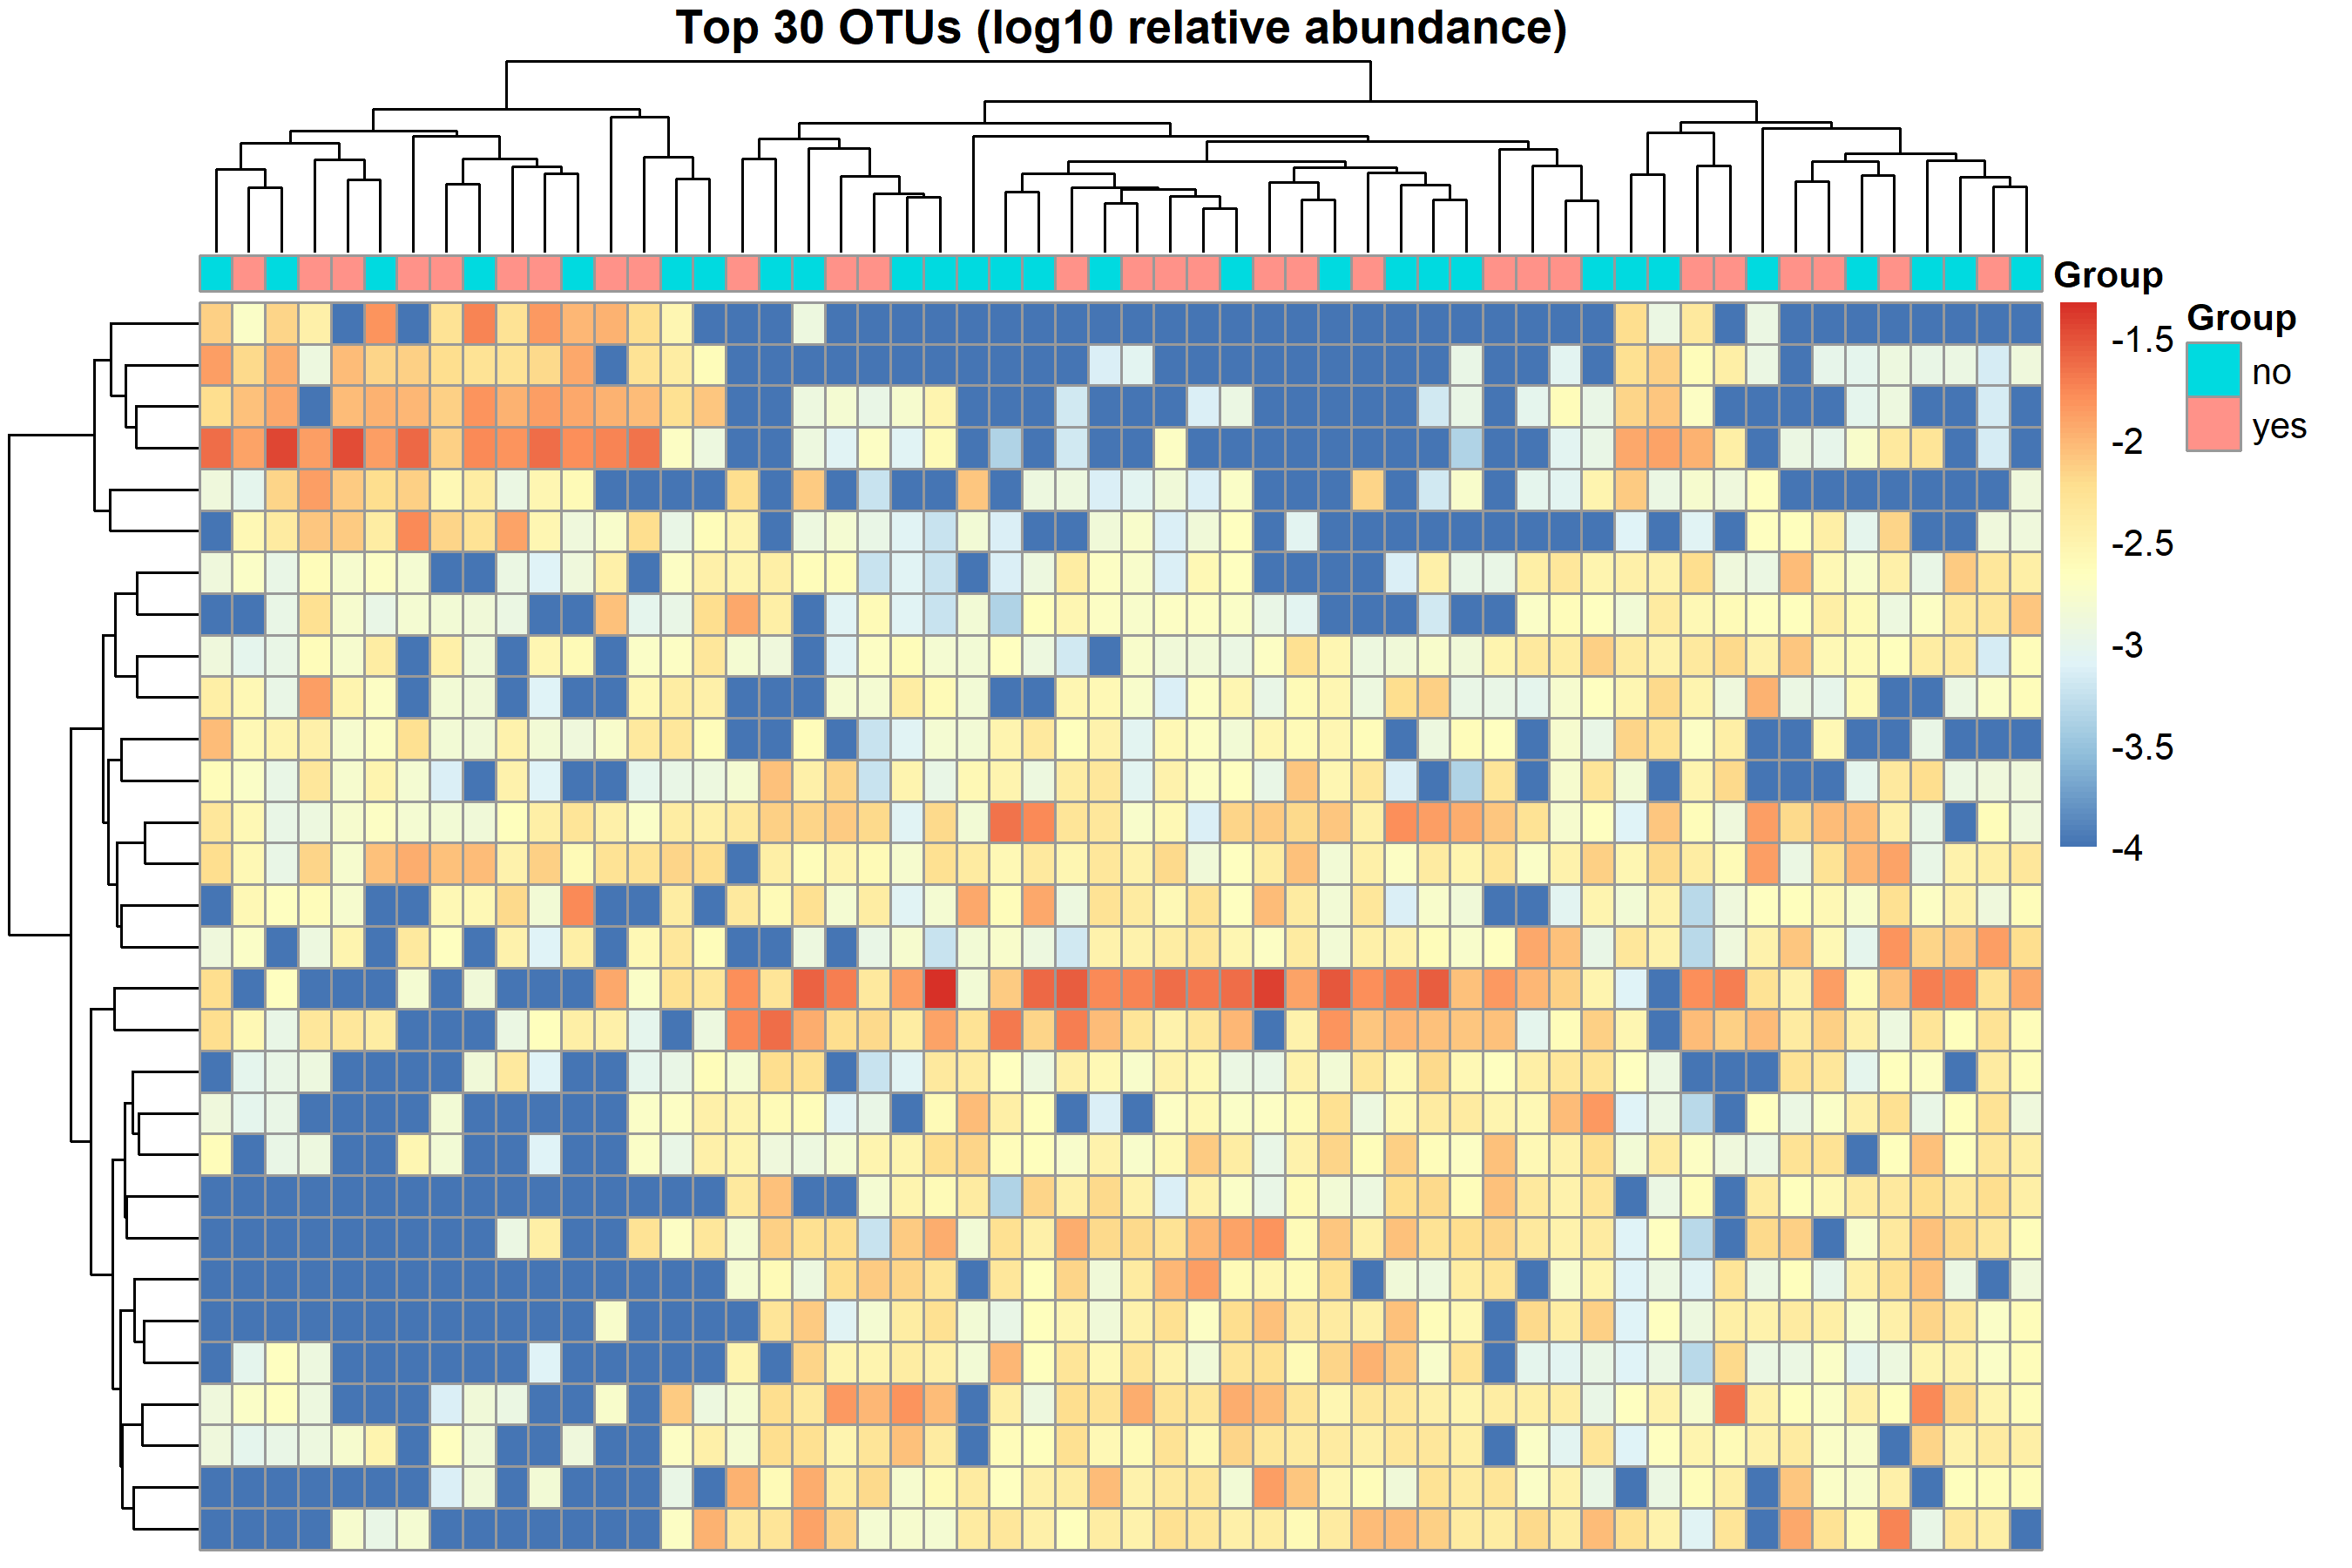
\includegraphics[keepaspectratio]{../figures/fig3_heatmap.png}}

\section{4. Main analysis}\label{main-analysis}

\subsection{4.1 Alpha diversity}\label{alpha-diversity}

\begin{Shaded}
\begin{Highlighting}[]
\CommentTok{\# Use raw (unpruned) counts, as recommended for richness estimators}
\NormalTok{alpha }\OtherTok{\textless{}{-}} \FunctionTok{estimate\_richness}\NormalTok{(soilrep, }\AttributeTok{measures =} \FunctionTok{c}\NormalTok{(}\StringTok{"Observed"}\NormalTok{, }\StringTok{"Shannon"}\NormalTok{, }\StringTok{"Simpson"}\NormalTok{))}
\NormalTok{alpha}\SpecialCharTok{$}\NormalTok{Group }\OtherTok{\textless{}{-}} \FunctionTok{sample\_data}\NormalTok{(soilrep)[[group\_var]]}
\NormalTok{alpha}\SpecialCharTok{$}\NormalTok{Sample }\OtherTok{\textless{}{-}} \FunctionTok{rownames}\NormalTok{(alpha)}

\NormalTok{alpha\_long }\OtherTok{\textless{}{-}}\NormalTok{ alpha }\SpecialCharTok{\%\textgreater{}\%}
  \FunctionTok{pivot\_longer}\NormalTok{(}\FunctionTok{c}\NormalTok{(Observed, Shannon, Simpson), }\AttributeTok{names\_to =} \StringTok{"Measure"}\NormalTok{, }\AttributeTok{values\_to =} \StringTok{"Value"}\NormalTok{)}

\NormalTok{p\_alpha }\OtherTok{\textless{}{-}} \FunctionTok{ggplot}\NormalTok{(alpha\_long, }\FunctionTok{aes}\NormalTok{(}\AttributeTok{x =}\NormalTok{ Group, }\AttributeTok{y =}\NormalTok{ Value, }\AttributeTok{fill =}\NormalTok{ Group)) }\SpecialCharTok{+}
  \FunctionTok{geom\_boxplot}\NormalTok{(}\AttributeTok{alpha =} \FloatTok{0.6}\NormalTok{, }\AttributeTok{outlier.shape =} \ConstantTok{NA}\NormalTok{) }\SpecialCharTok{+}
  \FunctionTok{geom\_jitter}\NormalTok{(}\AttributeTok{width =} \FloatTok{0.15}\NormalTok{, }\AttributeTok{size =} \FloatTok{1.5}\NormalTok{) }\SpecialCharTok{+}
  \FunctionTok{facet\_wrap}\NormalTok{(}\SpecialCharTok{\textasciitilde{}}\NormalTok{Measure, }\AttributeTok{scales =} \StringTok{"free\_y"}\NormalTok{) }\SpecialCharTok{+}
  \FunctionTok{labs}\NormalTok{(}\AttributeTok{title =} \StringTok{"Alpha diversity by group"}\NormalTok{, }\AttributeTok{x =} \ConstantTok{NULL}\NormalTok{, }\AttributeTok{y =} \StringTok{"Diversity value"}\NormalTok{) }\SpecialCharTok{+}
  \FunctionTok{theme\_minimal}\NormalTok{() }\SpecialCharTok{+} \FunctionTok{theme}\NormalTok{(}\AttributeTok{legend.position =} \StringTok{"none"}\NormalTok{)}
\NormalTok{p\_alpha}
\end{Highlighting}
\end{Shaded}

\pandocbounded{\includegraphics[keepaspectratio]{analysis_files/figure-latex/alpha-1.pdf}}

\begin{Shaded}
\begin{Highlighting}[]
\FunctionTok{ggsave}\NormalTok{(}\StringTok{"../figures/fig4\_alpha.png"}\NormalTok{, p\_alpha, }\AttributeTok{width =} \DecValTok{8}\NormalTok{, }\AttributeTok{height =} \DecValTok{4}\NormalTok{)}

\CommentTok{\# Kruskal{-}Wallis test: non{-}parametric, works for 2 or more groups}
\CommentTok{\# (with exactly 2 groups it is equivalent to the Wilcoxon rank{-}sum test)}
\NormalTok{alpha\_tests }\OtherTok{\textless{}{-}}\NormalTok{ alpha\_long }\SpecialCharTok{\%\textgreater{}\%}
  \FunctionTok{group\_by}\NormalTok{(Measure) }\SpecialCharTok{\%\textgreater{}\%}
  \FunctionTok{summarise}\NormalTok{(}\AttributeTok{p\_value =} \FunctionTok{kruskal.test}\NormalTok{(Value }\SpecialCharTok{\textasciitilde{}} \FunctionTok{factor}\NormalTok{(Group))}\SpecialCharTok{$}\NormalTok{p.value, }\AttributeTok{.groups =} \StringTok{"drop"}\NormalTok{) }\SpecialCharTok{\%\textgreater{}\%}
  \FunctionTok{mutate}\NormalTok{(}\AttributeTok{p\_adj =} \FunctionTok{p.adjust}\NormalTok{(p\_value, }\AttributeTok{method =} \StringTok{"BH"}\NormalTok{))}
\NormalTok{alpha\_tests}
\end{Highlighting}
\end{Shaded}

\begin{verbatim}
## # A tibble: 3 x 3
##   Measure  p_value p_adj
##   <chr>      <dbl> <dbl>
## 1 Observed   0.928 0.928
## 2 Shannon    0.731 0.928
## 3 Simpson    0.491 0.928
\end{verbatim}

\begin{Shaded}
\begin{Highlighting}[]
\FunctionTok{write.csv}\NormalTok{(alpha\_tests, }\StringTok{"../results/alpha\_tests.csv"}\NormalTok{, }\AttributeTok{row.names =} \ConstantTok{FALSE}\NormalTok{)}
\end{Highlighting}
\end{Shaded}

\subsection{4.2 Beta diversity (Bray-Curtis, PCoA,
PERMANOVA)}\label{beta-diversity-bray-curtis-pcoa-permanova}

\begin{Shaded}
\begin{Highlighting}[]
\CommentTok{\# phyloseq:: prefix needed, because IRanges (loaded with DESeq2) also has a \textquotesingle{}distance\textquotesingle{} function}
\NormalTok{bray }\OtherTok{\textless{}{-}}\NormalTok{ phyloseq}\SpecialCharTok{::}\FunctionTok{distance}\NormalTok{(ps\_rel, }\AttributeTok{method =} \StringTok{"bray"}\NormalTok{)}
\NormalTok{ord  }\OtherTok{\textless{}{-}} \FunctionTok{ordinate}\NormalTok{(ps\_rel, }\AttributeTok{method =} \StringTok{"PCoA"}\NormalTok{, }\AttributeTok{distance =}\NormalTok{ bray)}

\NormalTok{p\_pcoa }\OtherTok{\textless{}{-}} \FunctionTok{plot\_ordination}\NormalTok{(ps\_rel, ord, }\AttributeTok{color =}\NormalTok{ group\_var) }\SpecialCharTok{+}
  \FunctionTok{stat\_ellipse}\NormalTok{(}\AttributeTok{level =} \FloatTok{0.9}\NormalTok{) }\SpecialCharTok{+}
  \FunctionTok{labs}\NormalTok{(}\AttributeTok{title =} \StringTok{"PCoA of Bray{-}Curtis dissimilarity"}\NormalTok{) }\SpecialCharTok{+}
  \FunctionTok{theme\_minimal}\NormalTok{()}
\NormalTok{p\_pcoa}
\end{Highlighting}
\end{Shaded}

\pandocbounded{\includegraphics[keepaspectratio]{analysis_files/figure-latex/beta-1.pdf}}

\begin{Shaded}
\begin{Highlighting}[]
\FunctionTok{ggsave}\NormalTok{(}\StringTok{"../figures/fig5\_pcoa.png"}\NormalTok{, p\_pcoa, }\AttributeTok{width =} \DecValTok{7}\NormalTok{, }\AttributeTok{height =} \DecValTok{5}\NormalTok{)}

\CommentTok{\# PERMANOVA: do group centroids differ?}
\NormalTok{meta }\OtherTok{\textless{}{-}} \FunctionTok{data.frame}\NormalTok{(}\FunctionTok{sample\_data}\NormalTok{(ps\_rel))}
\NormalTok{perm }\OtherTok{\textless{}{-}} \FunctionTok{adonis2}\NormalTok{(bray }\SpecialCharTok{\textasciitilde{}}\NormalTok{ meta[[group\_var]], }\AttributeTok{permutations =} \DecValTok{999}\NormalTok{)}
\NormalTok{perm}
\end{Highlighting}
\end{Shaded}

\begin{verbatim}
## Permutation test for adonis under reduced model
## Permutation: free
## Number of permutations: 999
## 
## adonis2(formula = bray ~ meta[[group_var]], permutations = 999)
##          Df SumOfSqs      R2      F Pr(>F)
## Model     1   0.3291 0.01835 1.0092  0.324
## Residual 54  17.6084 0.98165              
## Total    55  17.9374 1.00000
\end{verbatim}

\begin{Shaded}
\begin{Highlighting}[]
\CommentTok{\# PERMANOVA assumes similar dispersion between groups {-}\textgreater{} check}
\NormalTok{disp }\OtherTok{\textless{}{-}} \FunctionTok{betadisper}\NormalTok{(bray, meta[[group\_var]])}
\FunctionTok{anova}\NormalTok{(disp)}
\end{Highlighting}
\end{Shaded}

\begin{verbatim}
## Analysis of Variance Table
## 
## Response: Distances
##           Df   Sum Sq   Mean Sq F value Pr(>F)
## Groups     1 0.000091 9.082e-05  0.0583 0.8101
## Residuals 54 0.084131 1.558e-03
\end{verbatim}

\subsection{4.3 Differential abundance
(DESeq2)}\label{differential-abundance-deseq2}

\begin{Shaded}
\begin{Highlighting}[]
\CommentTok{\# Convert phyloseq {-}\textgreater{} DESeq2 (raw counts, pruned OTUs)}
\NormalTok{dds }\OtherTok{\textless{}{-}} \FunctionTok{phyloseq\_to\_deseq2}\NormalTok{(ps, }\FunctionTok{as.formula}\NormalTok{(}\FunctionTok{paste}\NormalTok{(}\StringTok{"\textasciitilde{}"}\NormalTok{, group\_var)))}

\CommentTok{\# \textquotesingle{}poscounts\textquotesingle{} size factors handle the many zeros in microbiome data}
\NormalTok{dds }\OtherTok{\textless{}{-}} \FunctionTok{estimateSizeFactors}\NormalTok{(dds, }\AttributeTok{type =} \StringTok{"poscounts"}\NormalTok{)}
\NormalTok{dds }\OtherTok{\textless{}{-}} \FunctionTok{DESeq}\NormalTok{(dds, }\AttributeTok{fitType =} \StringTok{"local"}\NormalTok{)}

\CommentTok{\# With more than 2 groups DESeq2 needs to know WHICH two to compare.}
\CommentTok{\# By default: 2nd level vs 1st level. Change these two lines if you want another pair.}
\NormalTok{lev }\OtherTok{\textless{}{-}} \FunctionTok{levels}\NormalTok{(}\FunctionTok{factor}\NormalTok{(}\FunctionTok{sample\_data}\NormalTok{(ps)[[group\_var]]))}
\FunctionTok{print}\NormalTok{(lev)}
\end{Highlighting}
\end{Shaded}

\begin{verbatim}
## [1] "no"  "yes"
\end{verbatim}

\begin{Shaded}
\begin{Highlighting}[]
\NormalTok{reference  }\OtherTok{\textless{}{-}}\NormalTok{ lev[}\DecValTok{1}\NormalTok{]}
\NormalTok{comparison }\OtherTok{\textless{}{-}}\NormalTok{ lev[}\DecValTok{2}\NormalTok{]}
\FunctionTok{cat}\NormalTok{(}\StringTok{"Comparing"}\NormalTok{, comparison, }\StringTok{"vs"}\NormalTok{, reference, }\StringTok{"}\SpecialCharTok{\textbackslash{}n}\StringTok{"}\NormalTok{)}
\end{Highlighting}
\end{Shaded}

\begin{verbatim}
## Comparing yes vs no
\end{verbatim}

\begin{Shaded}
\begin{Highlighting}[]
\NormalTok{res }\OtherTok{\textless{}{-}} \FunctionTok{results}\NormalTok{(dds, }\AttributeTok{contrast =} \FunctionTok{c}\NormalTok{(group\_var, comparison, reference), }\AttributeTok{alpha =} \FloatTok{0.05}\NormalTok{)}
\NormalTok{res\_df }\OtherTok{\textless{}{-}} \FunctionTok{as.data.frame}\NormalTok{(res) }\SpecialCharTok{\%\textgreater{}\%}
  \FunctionTok{rownames\_to\_column}\NormalTok{(}\StringTok{"OTU"}\NormalTok{) }\SpecialCharTok{\%\textgreater{}\%}
  \FunctionTok{filter}\NormalTok{(}\SpecialCharTok{!}\FunctionTok{is.na}\NormalTok{(padj))}

\CommentTok{\# Add taxonomy only if it exists}
\NormalTok{has\_tax }\OtherTok{\textless{}{-}} \SpecialCharTok{!}\FunctionTok{is.null}\NormalTok{(}\FunctionTok{tax\_table}\NormalTok{(ps, }\AttributeTok{errorIfNULL =} \ConstantTok{FALSE}\NormalTok{))}
\ControlFlowTok{if}\NormalTok{ (has\_tax) \{}
\NormalTok{  tax }\OtherTok{\textless{}{-}} \FunctionTok{as.data.frame}\NormalTok{(}\FunctionTok{tax\_table}\NormalTok{(ps)) }\SpecialCharTok{\%\textgreater{}\%} \FunctionTok{rownames\_to\_column}\NormalTok{(}\StringTok{"OTU"}\NormalTok{)}
\NormalTok{  res\_df }\OtherTok{\textless{}{-}} \FunctionTok{left\_join}\NormalTok{(res\_df, tax, }\AttributeTok{by =} \StringTok{"OTU"}\NormalTok{)}
\NormalTok{\}}
\NormalTok{res\_df }\OtherTok{\textless{}{-}}\NormalTok{ res\_df }\SpecialCharTok{\%\textgreater{}\%} \FunctionTok{arrange}\NormalTok{(padj)}

\NormalTok{sig }\OtherTok{\textless{}{-}}\NormalTok{ res\_df }\SpecialCharTok{\%\textgreater{}\%} \FunctionTok{filter}\NormalTok{(padj }\SpecialCharTok{\textless{}} \FloatTok{0.05}\NormalTok{)}
\FunctionTok{cat}\NormalTok{(}\StringTok{"Significant OTUs (FDR \textless{} 0.05):"}\NormalTok{, }\FunctionTok{nrow}\NormalTok{(sig), }\StringTok{"}\SpecialCharTok{\textbackslash{}n}\StringTok{"}\NormalTok{)}
\end{Highlighting}
\end{Shaded}

\begin{verbatim}
## Significant OTUs (FDR < 0.05): 0
\end{verbatim}

\begin{Shaded}
\begin{Highlighting}[]
\FunctionTok{head}\NormalTok{(sig, }\DecValTok{15}\NormalTok{)}
\end{Highlighting}
\end{Shaded}

\begin{verbatim}
## [1] OTU            baseMean       log2FoldChange lfcSE          stat          
## [6] pvalue         padj          
## <0 rows> (or 0-length row.names)
\end{verbatim}

\begin{Shaded}
\begin{Highlighting}[]
\FunctionTok{write.csv}\NormalTok{(res\_df, }\StringTok{"../results/deseq2\_results.csv"}\NormalTok{, }\AttributeTok{row.names =} \ConstantTok{FALSE}\NormalTok{)}

\CommentTok{\# Volcano plot}
\NormalTok{res\_df}\SpecialCharTok{$}\NormalTok{Significant }\OtherTok{\textless{}{-}}\NormalTok{ res\_df}\SpecialCharTok{$}\NormalTok{padj }\SpecialCharTok{\textless{}} \FloatTok{0.05}
\NormalTok{p\_volcano }\OtherTok{\textless{}{-}} \FunctionTok{ggplot}\NormalTok{(res\_df, }\FunctionTok{aes}\NormalTok{(log2FoldChange, }\SpecialCharTok{{-}}\FunctionTok{log10}\NormalTok{(padj), }\AttributeTok{colour =}\NormalTok{ Significant)) }\SpecialCharTok{+}
  \FunctionTok{geom\_point}\NormalTok{(}\AttributeTok{alpha =} \FloatTok{0.6}\NormalTok{) }\SpecialCharTok{+}
  \FunctionTok{scale\_colour\_manual}\NormalTok{(}\AttributeTok{values =} \FunctionTok{c}\NormalTok{(}\StringTok{"grey60"}\NormalTok{, }\StringTok{"firebrick"}\NormalTok{)) }\SpecialCharTok{+}
  \FunctionTok{geom\_hline}\NormalTok{(}\AttributeTok{yintercept =} \SpecialCharTok{{-}}\FunctionTok{log10}\NormalTok{(}\FloatTok{0.05}\NormalTok{), }\AttributeTok{linetype =} \StringTok{"dashed"}\NormalTok{) }\SpecialCharTok{+}
  \FunctionTok{labs}\NormalTok{(}\AttributeTok{title =} \StringTok{"Differentially abundant OTUs (DESeq2)"}\NormalTok{,}
       \AttributeTok{x =} \StringTok{"log2 fold change"}\NormalTok{, }\AttributeTok{y =} \StringTok{"{-}log10 adjusted p{-}value"}\NormalTok{) }\SpecialCharTok{+}
  \FunctionTok{theme\_minimal}\NormalTok{()}
\NormalTok{p\_volcano}
\end{Highlighting}
\end{Shaded}

\pandocbounded{\includegraphics[keepaspectratio]{analysis_files/figure-latex/deseq-1.pdf}}

\begin{Shaded}
\begin{Highlighting}[]
\FunctionTok{ggsave}\NormalTok{(}\StringTok{"../figures/fig6\_volcano.png"}\NormalTok{, p\_volcano, }\AttributeTok{width =} \DecValTok{7}\NormalTok{, }\AttributeTok{height =} \DecValTok{5}\NormalTok{)}

\CommentTok{\# Which phyla do significant OTUs belong to?}
\ControlFlowTok{if}\NormalTok{ (}\FunctionTok{nrow}\NormalTok{(sig) }\SpecialCharTok{\textgreater{}} \DecValTok{0} \SpecialCharTok{\&\&}\NormalTok{ has\_tax) \{}
\NormalTok{  p\_phyla }\OtherTok{\textless{}{-}}\NormalTok{ sig }\SpecialCharTok{\%\textgreater{}\%}
    \FunctionTok{mutate}\NormalTok{(}\AttributeTok{Phylum =} \FunctionTok{ifelse}\NormalTok{(}\FunctionTok{is.na}\NormalTok{(Phylum), }\StringTok{"Unclassified"}\NormalTok{, Phylum)) }\SpecialCharTok{\%\textgreater{}\%}
    \FunctionTok{ggplot}\NormalTok{(}\FunctionTok{aes}\NormalTok{(}\AttributeTok{x =} \FunctionTok{reorder}\NormalTok{(Phylum, log2FoldChange, }\AttributeTok{FUN =}\NormalTok{ median),}
               \AttributeTok{y =}\NormalTok{ log2FoldChange, }\AttributeTok{colour =}\NormalTok{ Phylum)) }\SpecialCharTok{+}
    \FunctionTok{geom\_jitter}\NormalTok{(}\AttributeTok{width =} \FloatTok{0.1}\NormalTok{, }\AttributeTok{size =} \DecValTok{2}\NormalTok{) }\SpecialCharTok{+} \FunctionTok{coord\_flip}\NormalTok{() }\SpecialCharTok{+}
    \FunctionTok{geom\_hline}\NormalTok{(}\AttributeTok{yintercept =} \DecValTok{0}\NormalTok{, }\AttributeTok{linetype =} \StringTok{"dashed"}\NormalTok{) }\SpecialCharTok{+}
    \FunctionTok{labs}\NormalTok{(}\AttributeTok{title =} \StringTok{"Significant OTUs by phylum"}\NormalTok{, }\AttributeTok{x =} \ConstantTok{NULL}\NormalTok{, }\AttributeTok{y =} \StringTok{"log2 fold change"}\NormalTok{) }\SpecialCharTok{+}
    \FunctionTok{theme\_minimal}\NormalTok{() }\SpecialCharTok{+} \FunctionTok{theme}\NormalTok{(}\AttributeTok{legend.position =} \StringTok{"none"}\NormalTok{)}
  \FunctionTok{print}\NormalTok{(p\_phyla)}
  \FunctionTok{ggsave}\NormalTok{(}\StringTok{"../figures/fig7\_sig\_phyla.png"}\NormalTok{, p\_phyla, }\AttributeTok{width =} \DecValTok{7}\NormalTok{, }\AttributeTok{height =} \DecValTok{5}\NormalTok{)}
\NormalTok{\}}
\end{Highlighting}
\end{Shaded}

\section{5. Interpretation notes (use in
README)}\label{interpretation-notes-use-in-readme}

\begin{itemize}
\tightlist
\item
  Alpha diversity: see \texttt{alpha\_tests} (is richness/diversity
  different between groups?).
\item
  Beta diversity: PERMANOVA R2 = how much community variation the group
  explains; check the dispersion test before trusting it.
\item
  DESeq2: positive log2FoldChange means higher abundance in the
  non-reference group (check \texttt{resultsNames(dds)}).
\item
  Limitations: small sample size, OTU-based 16S data (genus-level
  resolution only), observational association not mechanism.
\end{itemize}

\section{6. Session info (for the Reproducibility
section)}\label{session-info-for-the-reproducibility-section}

\begin{Shaded}
\begin{Highlighting}[]
\FunctionTok{sessionInfo}\NormalTok{()}
\end{Highlighting}
\end{Shaded}

\begin{verbatim}
## R version 4.6.2 (2026-10-29 ucrt)
## Platform: x86_64-w64-mingw32/x64
## Running under: Windows 11 x64 (build 26100)
## 
## Matrix products: default
##   LAPACK version 3.12.1
## 
## locale:
## [1] LC_COLLATE=English_United Kingdom.utf8 
## [2] LC_CTYPE=English_United Kingdom.utf8   
## [3] LC_MONETARY=English_United Kingdom.utf8
## [4] LC_NUMERIC=C                           
## [5] LC_TIME=English_United Kingdom.utf8    
## 
## time zone: Asia/Colombo
## tzcode source: internal
## 
## attached base packages:
## [1] stats4    stats     graphics  grDevices utils     datasets  methods  
## [8] base     
## 
## other attached packages:
##  [1] pheatmap_1.0.13             lubridate_1.9.5            
##  [3] forcats_1.0.1               stringr_1.6.0              
##  [5] dplyr_1.2.1                 purrr_1.2.2                
##  [7] readr_2.2.0                 tidyr_1.3.2                
##  [9] tibble_3.3.1                ggplot2_4.0.3              
## [11] tidyverse_2.0.0             vegan_2.7-6                
## [13] permute_0.10-0              DESeq2_1.52.0              
## [15] SummarizedExperiment_1.42.0 Biobase_2.72.0             
## [17] MatrixGenerics_1.24.0       matrixStats_1.5.0          
## [19] GenomicRanges_1.64.0        Seqinfo_1.2.0              
## [21] IRanges_2.46.0              S4Vectors_0.50.3           
## [23] BiocGenerics_0.58.1         generics_0.1.4             
## [25] phyloseq_1.56.0            
## 
## loaded via a namespace (and not attached):
##  [1] ade4_1.7-24         tidyselect_1.2.1    farver_2.1.2       
##  [4] Biostrings_2.80.2   S7_0.2.2            fastmap_1.2.0      
##  [7] digest_0.6.39       timechange_0.4.0    lifecycle_1.0.5    
## [10] cluster_2.1.8.3     survival_3.8-12     magrittr_2.0.5     
## [13] compiler_4.6.2      rlang_1.3.0         tools_4.6.2        
## [16] utf8_1.2.6          igraph_2.3.4        yaml_2.3.12        
## [19] data.table_1.18.6.1 knitr_1.52          labeling_0.4.3     
## [22] S4Arrays_1.12.1     DelayedArray_0.38.2 plyr_1.8.9         
## [25] RColorBrewer_1.1-3  abind_1.4-8         BiocParallel_1.46.0
## [28] withr_3.0.3         grid_4.6.2          multtest_2.68.0    
## [31] biomformat_1.40.0   scales_1.4.0        iterators_1.0.14   
## [34] MASS_7.3-66         cli_3.6.6           rmarkdown_2.32     
## [37] crayon_1.5.3        ragg_1.5.2          otel_0.3.0         
## [40] rstudioapi_0.19.0   reshape2_1.4.5      tzdb_0.5.0         
## [43] ape_5.8-1           splines_4.6.2       parallel_4.6.2     
## [46] XVector_0.52.0      vctrs_0.7.3         Matrix_1.7-6       
## [49] jsonlite_2.0.0      hms_1.1.4           systemfonts_1.3.2  
## [52] locfit_1.5-9.12     foreach_1.5.2       glue_1.8.1         
## [55] codetools_0.2-20    stringi_1.8.9       gtable_0.3.6       
## [58] pillar_1.11.1       htmltools_0.5.9     R6_2.6.1           
## [61] textshaping_1.0.5   evaluate_1.0.5      lattice_0.23-1     
## [64] Rcpp_1.1.2          SparseArray_1.12.3  nlme_3.1-171       
## [67] mgcv_1.9-4          xfun_0.62           pkgconfig_2.0.3
\end{verbatim}

\end{document}
